Η υλοποίηση C στο περιβάλλον ESP-IDF είναι ιδιαίτερα εύκολη καθώς οι
περισσότερες βιβλιοθήκες είναι ενσωματωμένες στο build system που
προσφέρει η Espressif. Συγκεκριμένα οι βιβλιοθήκες που μας ενδιαφέρουν και
είναι έτοιμες να γίνουν include μετά το setup είναι:

\begin{enumerate}
        \item Η υλοποίηση FreeRTOS.
        \item H υλοποίηση του MQTTV5.
        \item Η βιβλιοθήκη για WiFi.
\end{enumerate}

Μας λοίπει δηλαδή:

\begin{enumerate}
        \item Μια βιβλιοθήκη για διαχείριση του HCSR04.
        \item Μια βιβλιοθήκη για δημιουργία JSON.
\end{enumerate}

Προτεινόμενος τρόπος να ξεκινήσουμε ένα
project είναι να αντιγράψουμε ένα template από το repository
του esp-idf.

\begin{lstlisting}
git clone https://github.com/espressif/esp-idf
mkdir my-project
cp $ESP_IDF_PATH/examples/$MY_TEMPLATE  my-project/
\end{lstlisting}

Έπειτα κάνουμε source τα python scripts που μας βοηθάνε
να κάνουμε build, flash και monitor. Τα python scripts
μόλις γίνουν source γίνονται ορατά στον χρήστη και συνήθως
χρησιμοποιούμε το \verb|idf.py| ως το κύριο πρόγραμμα
για να τα τρέξουμε.

\begin{lstlisting}
. $ESP_IDF_PATH/export.sh
\end{lstlisting}

Μπορούμε πλέον να δημιουργήσουμε τα απαραίτητα αρχεία 
στα οποία θα γραφτεί ο κώδικας. Η εικόνα \ref{fig:idf_filestructure}
παρουσιάζει την δομή των αρχείων του project χωρίς τις βιβλιοθήκες.

\begin{figure}[!htb]
    \centering
    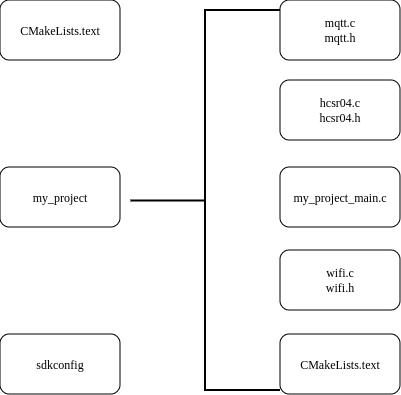
\includegraphics[scale=0.4]{images/espidf/idf-filestructure.png}
    \caption{Project filestructure}
    \label{fig:idf_filestructure}
\end{figure}

Το \verb|sdkconfig| είναι μια συλλογή από macros τα
οποία περνάνε ως flags στον compiler. Η χρησιμότητα τους
είναι κυρίως στην εξατομίκευση του προγράμματος και του
μικροελεγκτή. Μέσο αυτών μπορούμε να επιλέξουμε την ταχύτητα του
ρολογιού του επεξεργαστή, να ενεργοποιήσουμε ή να απενεργοποιήσουμε
hooks ή να φτιάξουμε τα δικά μας \verb|#defines| για διαφορετικές υλοποιήσεις
του ίδιου project. Προφανώς θα μπορούσαμε να κάνουμε όλα τα παραπάνω
προγραμματιστικά αλλά το sdkconfig προσφέρει ένα ωραίο interface μέσο
του \verb|idf.py menuconfig|. Χρησιμοποιώντας αυτό το interface εμείς
θέτουμε \verb|configUSE_IDLE_HOOK| ίσο με $1$ για να μπορούμε
να μετρήσουμε το idle time του επεξεργαστή.

Το \verb|CMakeLists| είναι απλώς το build script. Ο τρόπος με τον
οποίο το περιβάλλον ESP-IDF κατηγοριοποιεί ένα project είναι μέσο των
components, ουσιαστικά εξωτερικές βιβλιοθήκες. Οτιδήποτε δεν είναι
component θεωρείτε κύριος πηγαίος κώδικας και βρίσκεται στον φάκελο με
το όνομα του project. Η κατανοήσει του παραπάνω είναι σημαντική διότι
υπάρχουν δύο (τουλάχιστον) CMakeLists. Το build script που βρίσκεται
στην ρίζα του project και το build script που βρίσκεται στον φάκελο
που βρίσκεται ο πηγαίος κώδικας. To εξωτερικό build script είναι
υπεύθυνο για την ενσωμάτωση components και ορίζει το όνομα του project.
Για παράδειγμα εφόσον θέλουμε τουλάχιστον δύο έξτρα βιβλιοθήκες:

\begin{lstlisting}
cmake_minimum_required(VERSION 3.16)
set(EXTRA_COMPONENT_DIRS ./components/)
include($ENV{IDF_PATH}/tools/cmake/project.cmake)
project(my-project)
\end{lstlisting}

Δημιουργούμε το component directory και εκεί βάζουμε το source code των
libraries. Στην δικιά μας περίπτωση χρησιμοποιούμε το esp-idf-lib το οποίο
περιέχει ένα driver για τον HCSR04 και το CJSON για να δημιουργήσουμε JSON
strings.

Το εσωτερικό \verb|CMakeLists| περιέχει όλα τα αρχεία που έχουν
πηγαίο κώδικα:

\begin{lstlisting}
idf_component_register(SRCS "my_project_main.c"
                             "hcsr04.c"
			     "wifi.c"
			     "mqtt.c"
                    INCLUDE_DIRS "")
\end{lstlisting}

